\begin{frame}{Nécessité de la cohérence}
 \begin{columns}[T]
    \begin{column}{.4\textwidth}
    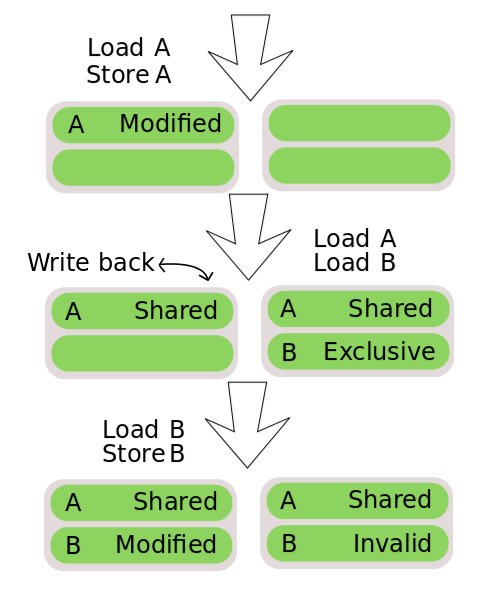
\includegraphics[scale=.3]{images/learn_mesi_2.png} 
    \end{column}
    \begin{column}{.6\textwidth}
      \begin{block}{Partage}
        Plusieurs caches peuvent contenir la même donnée lorsque celle-ci est lue.
      \end{block}
      \begin{block}{Modification}
        Lorsqu'un cache la modifie, il doit en informer les autres et éventuellement transmettre la nouvelle donnée.
      \end{block}
      \begin{block}{Messages}
        Pour informer les autres et transmettre, des messages sont envoyés entre les caches.
      \end{block}
    \end{column}
 \end{columns}
\end{frame}

\begin{frame}{Solution MESI}
  \begin{block}{Cohérence = automate}
    Les lignes de caches respectent certaines caractéristiques d'un automate : ont un nombre fini d'états, et passent de l'un à l'autre suivant des actions extérieurs (i.e. étiquettes/transitions).\\
    Pour \textsf{Cassis}, usage de \textsf{SMC} afin de représenter les automates de cohérences.
  \end{block}
  
  \begin{block}{Les états :}
    \begin{itemize}
    \item{I (donnée invalide),}
    \item{M (donnée modifiée),}
    \item{S (donnée partagée),}
    \item{E (donnée unique).}
    \end{itemize}
  \end{block}
\end{frame}

\begin{frame}{Automate MESI : les transitions}
    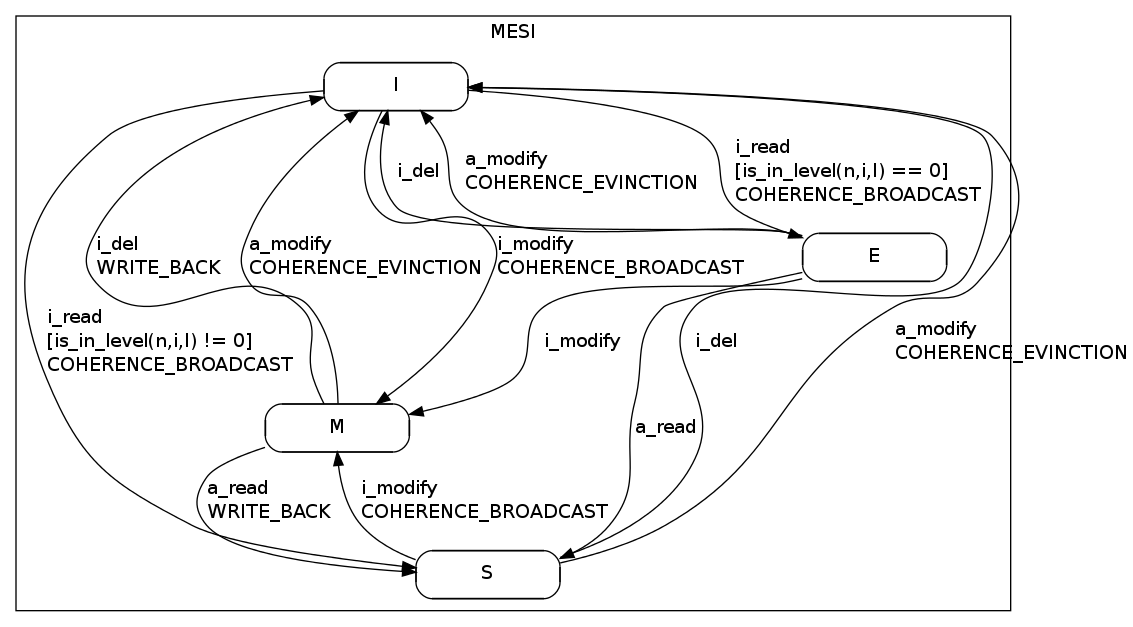
\includegraphics[scale=.3]{images/MESI_simple.png}
\end{frame}

\begin{frame}{Autres protocoles}
  \begin{block}{Protocoles implémentés}
    Les autres protocoles courants sont :
    \begin{itemize}
    \item{MSI (le plus basique),}
    \item{MOSI/MESIF (alternative presque équivalente à MESI),}
    \item{MOESI (le plus complexe).}
    \end{itemize}
  \end{block}
  
  \begin{block}{Avantages/Inconvénients}
    Deux critères importants pour le choix d'un protocole :
    \begin{itemize}
    \item{le nombre de \emph{write-back},}
    \item{l'utilisation de la bande-passante.}
    \end{itemize}
  \end{block}
\end{frame}

